\documentclass[arial,11pt]{article}
%\documentclass[11pt]{nih}
\usepackage[dvips]{graphicx}
\usepackage[colorlinks=true,linkcolor=black]{hyperref}
\usepackage{amssymb}
%\usepackage{graphicx}
%\usepackage{longtable}
\usepackage{epsfig}
%\usepackage{overcite}
\usepackage[usenames]{color}

\renewcommand{\rmdefault}{phv} % Arial
\renewcommand{\sfdefault}{phv} % Arial
\renewcommand{\thesection}{\Alph{section}}
\pagestyle{empty}

%\usepackage{times}
\usepackage{geometry}
%\geometry{tmargin=1in,bmargin=1.0in,lmargin=1in,rmargin=1in}
\geometry{tmargin=0.95in,bmargin=0.95in,lmargin=0.95in,rmargin=0.95in}
%\linespread{0.95} \interfootnotelinepenalty=10000

%%%%% editing helpers
\newcommand{\NeedRevision}[1]{\textcolor{red}{#1}}

\begin{document}

\begin{center}
{\Large  \bf{Driving Biomedical Project 3:\\  Interspecies chemical interactions


}}
\end{center}

\begin{itemize}
%\item {\bf Funding status of the project:}  funded
\item {\bf Collaborating investigator:}  Kit Pogliano/Pieter Dorrestein
\item {\bf Institution:} Division of Biological Sciences at UCSD/School of Pharmacy at UCSD
\item {\bf Funded project:} 	The chemical and genetic basis of interspecies interactions
\item {\bf Grant number:} 	5 R01 AI095125   	
\item {\bf Project period:}   4/1/2011 to 3/31/2015,
\item {\bf Agency:}  NIAID
\item {\bf TRD interactions:}  TRD2 (Antibiotics sequencing), TRD3 (Spectral networks) and TRD8 (ProteoSAFe/MassIVE).
\end{itemize}


%*******************************************
\section{Significance}
%*******************************************

%(1) Significance:
% address the importance as an impetus for TR&D of the biomedical research problem that will form the basis of the DBP;
% challenges inherent in this research problem that will drive TR&D;
% appropriateness of the DBP as a test-bed for technology being developed in the BTRC.

Metabolic exchange is a universal phenomenon that is essential to every organism from
%those as simple as
bacteria
%to complex higher eukaryotes such as
to humans. While metabolic exchange enables cooperation and coordination between
trillions of cells in a  human being, even unicellular organisms rely on metabolic exchange to adapt to environmental stress and form biofilms.
%Cellular communication allows stem cells to differentiate, cancer cells to proliferate, neurons to fire, bacteria to sense a quorum and pathogens to survive in %human hosts.
%
The chemical diversity of the molecules used for communication is extraordinary, and includes small ions, small molecules, fatty acids,  carbohydrates, peptides, proteins and nucleic acids. Despite the universal nature of metabolic exchange, there are few methods that can characterize the communication
between cells in a systematic and sensitive fashion, let alone real-time.
To achieve this goal, there is a need for both MSI studies of metabolic exchange (DBP9) and new approaches to analyze the biomolecules participating in metabolic exchange (this DBP).
In this DBP, the focus is on
%the application and adaptation of desorption electrospray mass spectrometry to enable
%the real-time live cell detection and
the spectral network visualization and characterization of metabolic exchange.
% in important biological processes.
%We aim to accomplish this in both a spatial as well as temporal fashion.
Supported by the algorithms  developed at CCMS, the experimental approaches developed in this DBP will improve our understanding of secreted biomarkers, microbiome-human cell interactions and
%understanding the complexities of
infectious diseases that derive from the cooperation between different types of cells (e.g. {\em Bacilli} with macrophages, neutrophils or T-cells).
% and interkingdom communication.
Ultimately,  it may drive the development of new therapeutic strategies
%or interventions
based on paradigms involving inter-cellular metabolic communication in a system wide fashion.

%Microbes use secreted factors to interact, communicate and manipulate their local environment and neighboring cell populations in a process known as metabolic exchange. By employing a wide breadth of molecules ranging from signaling compounds to defensive metabolites, metabolic exchange dictates not only basic microbial behavior such as biofilm formation, sporulation and motility, but also social interactions such as syntrophy and quorum sensing which enables microbes to establish communities.

Despite metabolic exchange having a major impact on the phenotypic development of microbial populations, there is a lack of tools that enable scientists to probe the chemistry of microbial colonies in a direct manner.
%, let alone of live microbial colonies.
Currently the chemistry of microbes is studied indirectly
% and, in general, on single molecules
and this effort comes with a significant time and monetary investment.
Drs. Pogliano and Dorrestein are developing tools that make this process more efficient and easier for non-chemists to study the chemistry of microbes as well as non-microbe cell populations.
These new experimental approaches will be  be easy to implement and  compatible with existing infrastructure.
%, and easily incorporated into future protocols,
Most importantly, they will provide information that current techniques cannot provide.
% and/or improve the ease by which this information is obtained and analyzed.
Furthermore, since organisms are not static entities, it is important that chemical exchanges be monitored temporally and spatially as both the timing of production and the distribution of metabolic exchange factors within microbial populations can provide valuable insights into the function of these molecules.

\begin{figure}[ht!]
%  \vspace{-20mm}
    \includegraphics[width=\textwidth]{figures/figNanoDESI.png}
%    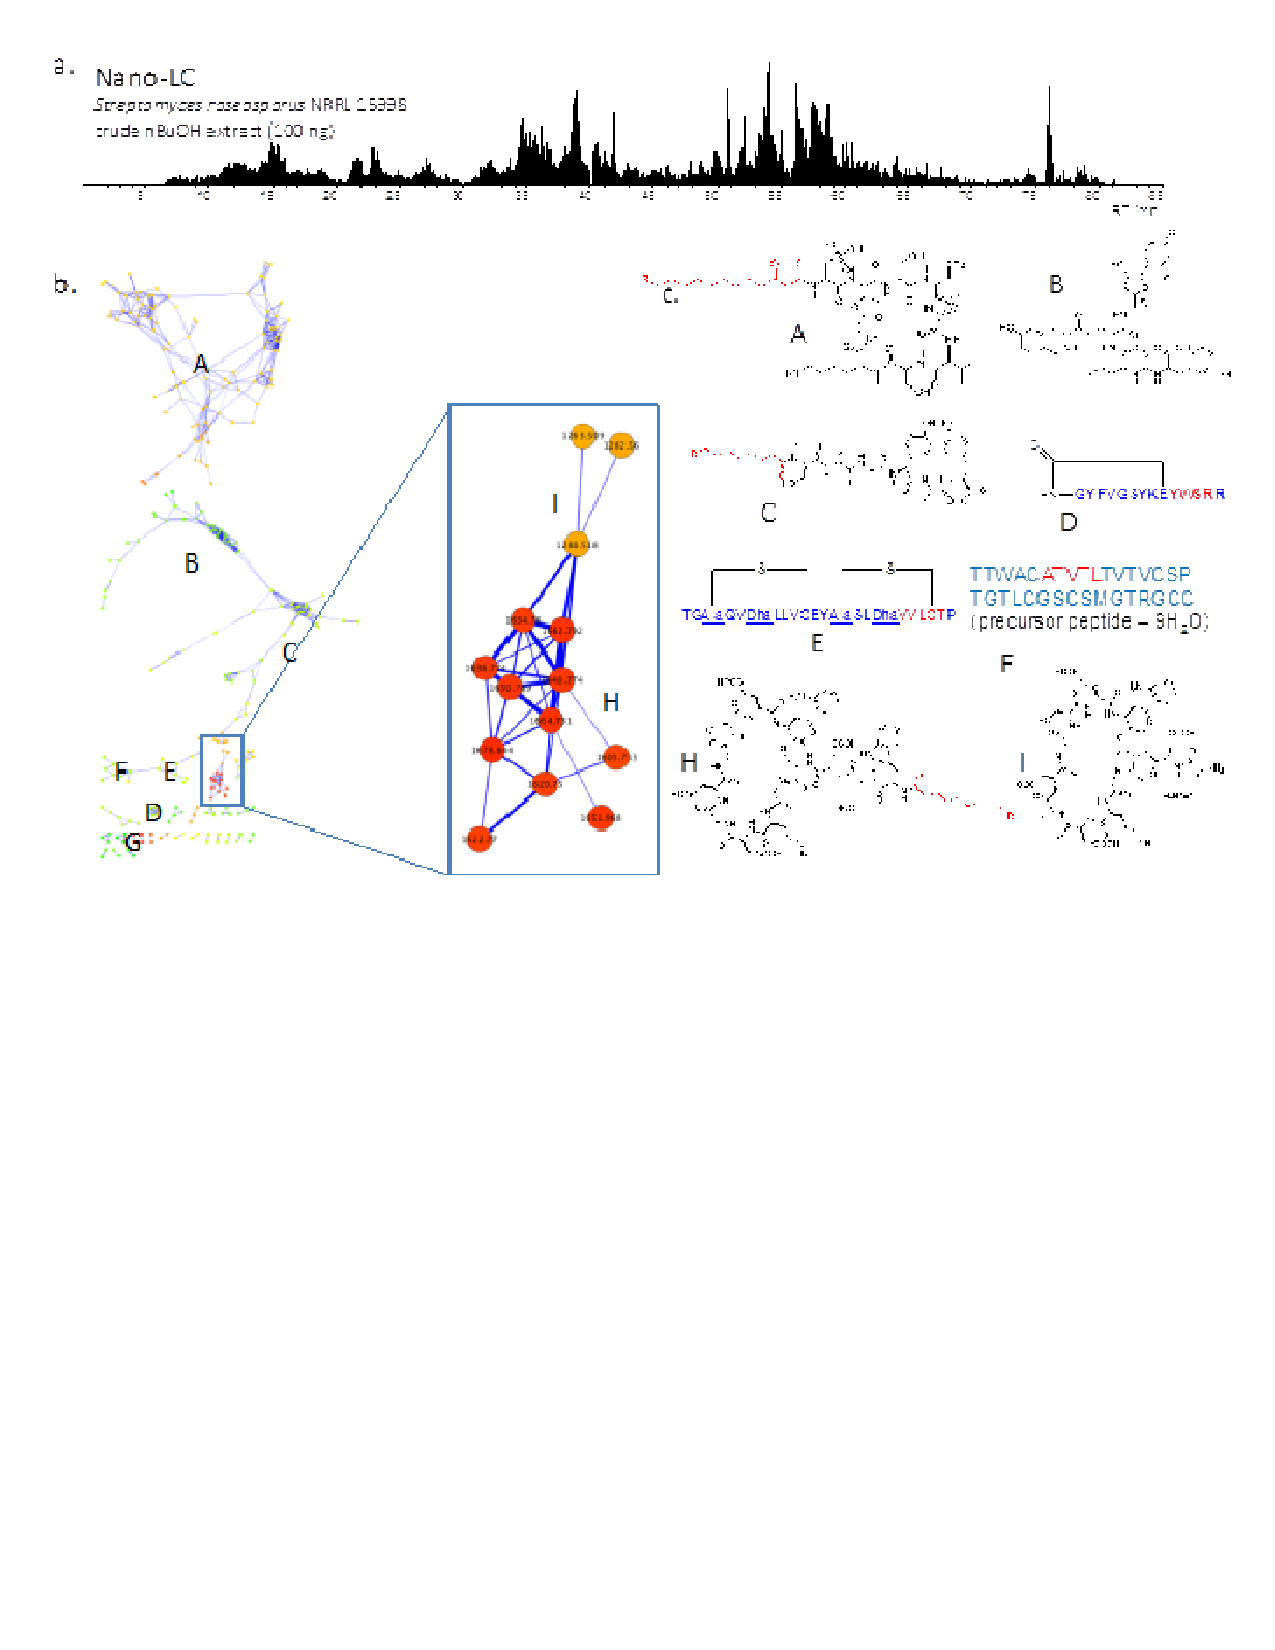
\includegraphics{figures/figApproach.png}
  \caption{\footnotesize   Monitoring microbial interactions with nanoDESI reveals communicating biomolecules. a) A schematic overview of nanoDESI. b) A photograph of the nanoDESI set-up with a microbial colony grown on an agar surface in a Petri dish. c) Time dependent analysis at a single location within a 3-day old {\em B. subtilis 3610} colony to indicate the changes in signal intensity of specific molecules over time. d) A mass spectrum obtained from a {\em B. subtilis 3610} colony with nanoDESI. *correspond to agar sugar signals, I is DGDG, II is lysyl-phosphatidylglycerol (LPG,) III is surfactin, IV is sublancin (3+), V is Sporulation killing factor (SKF) (2+), VI is plipastatin, VII is subtilosin (2+).}
  \label{fig.dbp.dorrestein.desi}
\end{figure}

With these goals in mind, this DBP will integrate  nanoDESI MS for chemical monitoring of living microbial populations
(Figure~\ref{fig.dbp.dorrestein.desi})
%in conjunction with $ii)$
with generation of spectral networks that enable one to visualize the observed molecules
%as nodes that represent a comparison of tandem mass spectrometry fragmentation data via spectral alignment
(Figure~\ref{fig.dbp.dorrestein.molnets}).  NanoDESI (see DBP9) and spectral networks (this DBP) provide a powerful new workflow for direct chemical analysis of secreted microbial exchange factors in live colonies. In preliminary studies~\cite{watrous12,moree12}, we have demonstrated the ability of spectral networks to temporally and spatially characterize single live microbial colonies as well as interacting microbes. This novel workflow provided unique insights into the extracellular chemistry of pathogenic microbes such as {\em Serratia sp.}, {\em Pseudomonas aeruginosa PA01}, and {\em Mycobacterium smegmatis MC2} as well as beneficial microbes such as {\em Pseudomonas sp. strain SH-C52} that protects from fungal infections. Spectral molecular networking of strain SH-C52 in conjunction with our peptidogenomic strategy have enabled the detection of thanamycin, a non-ribosomal peptide with antifungal activity.

%*******************************************
\section{Innovation}
%*******************************************

%(2) Innovation: Describe the innovations and technological advances that will result from the DBP interaction with Center TR&D and their implications beyond this project.

We can now sequence a single microbial genome in a few hours. However, connecting a single natural product molecule to its analogs and biosynthetic gene cluster often requires  several man-years of effort. The challenge tackled in this DBP is to make the discovery of microbial natural products compatible with the speed and efficiency that is now routine with microbial genome sequencing.

In collaboration with CCMS, this DBP will introduce MS methods and software that enable the mapping of molecules in structural and biosynthetic space. In effect, these tools will create an innovative GenBank-like paradigm geared for characterization of diverse molecules. Dozens of bacteria with and without sequenced genomes will be interrogated to generate a unique library of secondary metabolites and natural products. This  collaboration with CCMS will fine-tune a new set of computational tools with broad translational utility
% within many NIH priority areas
that use mass spectrometry (including metabolomics, lipidomics, peptidomics, and natural products research). We anticipate that this new paradigm will broadly impact  discovery of diverse communicated molecules to include new virulence factors and new therapeutic drugs.

%*******************************************
\section{Approach}
%*******************************************

%(3) Approach: Describe methods and procedures to be used, emphasizing the relationship between the DBP and BTRC personnel and technologies, rationale for the proposed approach to the problem and impact of the expertise of the BTRC investigators and technology on the project.

The goal of this DBP is to advance the field of natural products chemistry through the development and implementation of a new  molecular discovery paradigm much like the way GenBank, with its search engines such as BLAST, changed genomic sciences.
%Natural products are defined in this proposal as genetically encoded  molecules that drive cell signaling and cell differentiation.
Currently, natural product discovery and characterization is done one molecule at a time. This process is time consuming
%, at times taking years to identify a single molecule,
and requires a very high level of expertise, thereby limiting the study of a molecule's biological function. Mass spectrometry has the potential to dramatically transform these current practices by allowing for the rapid and unbiased exploration of any ionizable molecule. However, as most natural products are unique chemical entities limited to just one or a few organisms, there is currently no publicly available database that has a searchable MS/MS fragmentation library of sufficient size to cover the broad range of molecules produced by  known microbes. Moreover, even if such a database was available, current software does not support the type of approximate matching required to find related but polymorphic molecules. In addition, this database would not facilitate the discovery and characterization of novel molecules. Therefore, one has to typically resort to the manual interpretation of mass spectrometry data
%, which for a single MS/MS spectrum typically involves 10 minutes to several hours depending on its nature and complexity.
%This practice is obviously
that is very time consuming and becomes impractical when the data consist of thousands to millions of  spectra from hundreds of organisms. In the natural products research, such tools for data organization and navigation, let alone natural product identification, are nonexistent. Hence, alternative ways to look at MS data for natural products are needed.

This DBP focuses on a new approach based on the core principle that chemical/molecular similarity can be assessed by the similarity between tandem mass spectra of related molecules. In essence, this principle is the mass spectrometry equivalent of the fundamental comprative genomics principle that similar DNA sequences reveal related biological molecules and functions.
% (e.g., genes, motifs, protein/domain families, etc).
While this core {\em sequence similarity} principle continues to enable the genomics revolution, an analogous {\em spectral similarity} principle is only starting to be explored in natural products research.
% that now yields new complete genomes in just a few days and has made tools such as BLAST and GenBank indispensable in modern biology.

\begin{figure}[htb!]
%  \vspace{-20mm}
    \centering
    \includegraphics[width=.8\textwidth]{figures/figMolNets.png}
  \caption{\footnotesize  Molecular networks of nanoDESI fragmentation data obtained from microbial colonies. a) The annotated molecular network from {\em B. subtilis 3610}. b) The annotated molecular network of {\em Streptomyces coelicolor A3(2)}, {\em Mycobacterium smegmatis MC2}, {\em Pseudomonas aeruginosa PAO1}, {\em S. marcescens ES129}. The insets show images of the samples that were probed with nanoDESI. The coloring scale in this figure shows the mass range of the parent ions: green nodes represent the smallest masses all the way to red, which represent the largest masses fragmented. }
  \label{fig.dbp.dorrestein.molnets}
\end{figure}

The computational concepts for monitoring chemical interactions
%the required molecular spectral networks algorithms
are described in detail in TRD3 (spectral networks).
%In brief, pairs of MS/MS spectra from related molecules are first detected using spectral alignment to find spectra with significantly-similar fragmentation %patterns, regardless of whether the spectra are identified in advance or not. A perfect match is scored a $1$, while a no-match is given a value of $0$.
Molecular  networks will be  constructed by selecting significant spectrum matches (e.g., those with cosine scores $>0.5$) and representing them as edges (spectral alignments) connecting spectrum nodes.
It should be noted that while  the networks in Figure~\ref{fig.dbp.dorrestein.molnets} strongly support the feasibility of the proposed algorithms,
they are still mostly a visualization tool revealing the molecular diversity of biological samples.  Transforming this visualization tool into a robust discovery platform supporting natural products research will require the algorithmic developments proposed in TRD3 and TRD2 combined with efforts of the PIs in this DBP.  In addition, CCMS will collect the spectra and their identifications and will build a {\em natural products} section of MassIVE spectral depository (TRD8). Such public dataset of spectra and identifications of natural products  does not exist today and will be invaluable for future computational and experimental studies of natural products.

%To make this DBP successful, CCMS will develop
%tools for comparing
%%The four applications that will be developed in this DBP are the automated genome mining for natural products (TRD2) the comparison of
%two or more molecular networks (TRD3).
%%
%For example one may want to query whether an MS data set contains unique molecules that do not exist in the database. This is a query made possible with the comparative molecular networks approach.
%The progress of this DBP will result in future versions of this molecular network platform to include: 1) automated structure elucidation, 2) molecular phylogenetic  analysis, 3) the analysis of molecular changes of communities such as biofilms, 4) the comparison of disease vs. non disease states.
%%, and many other applications that are not possible with current scientific tools.
%The initial 250+ organism library to be analyzed by mass spectrometry includes common model organisms of general interest to the microbiology community.
% The results will be used to test the molecular network paradigm and use this approach to discover novel biomolecules that will be screened for therapeutic potential.


 CCMS has developed a molecular networking proof-of-concept software which is currently used as a tool for the visualization of MS data in all projects in Pieter Dorrestein's laboratory. The utility of this tool has been demonstrated with LC/MS/MS data from {\em Streptomyces roseosporus}, which is the industrial producer strain of the antibiotic daptomycin (\$700 million in annual sales). At the beginning of this project, daptomycin was the only reported natural product from this microbe. Using MS Imaging and spectral networks, we discovered four additional molecules:  arylomycin, an antibiotic under clinical evaluation by RQx Pharmaceuticals, two lantipeptides, and a lassopeptide. Analysis of our LC/MS/MS datasets that we previously collected for our peptidogenomics effort resulted in the molecular networks shown in Figure~\ref{fig.dbp.dorrestein.molnets}. This analysis revealed not only each of the molecules previously identified but also identified several sub-clusters representing previously unrecognized molecular entities. Upon further analysis aided by molecular networking, we characterized two subclusters as belonging to the antibiotic stenothricin and napsamycin families of natural products. In addition to previously characterized stenothricin and napsamycin molecules, we identified a series of novel analogues.

Although our proof-of concept molecular networks software  is functional, much algorithmic  and software development remains to be done (see TRD3). At present, the analysis is done manually after the molecular network is generated using only crude score thresholds of unknown statistical significance. As described in TRD3, we aim to automate these processes using improved algorithms and statistics. Additional spectral similarity scoring functions, spectral quality filters, and isotopic filters
%(e.g. if a node for the $^{12}C$ is displayed, the $^{13}C$ isotope fragmentation pattern is also displayed at this time)
need to be developed to significantly reduce the visual complexity of the molecular networks and allow the user to connect the molecule directly to the chemistry. Finally, subnetworks of unidentified molecules will be submitted for analysis with algorithms developed in TRD2 for antibiotics identification.



\paragraph{Impact of the expertise of the CCMS investigators on DBP.}
The spectral network paradigm that is crucial for this DBP was developed by  Drs. Bandeira and Pevzner.
Drs. Bandeira and Pevzner have been developing algorithms for
analyzing peptidic secondary metabolites via spectral networks and co-authored 16 papers with Dr. Dorrestein in 2009-2012 (including 2 papers with Dr. Pogliano).
In 2012, Drs. Bandeira, Dorrestein, and Pogliano demonstrated how molecular networks can be used for analyzing diverse molecules (not limited to peptides)  involved
in microbial interactions.

%%**************************************************************************************
%% ------------------------------------------------------------------------------------
%\section{Technology Research and Development projects (TR\&Ds)}
%% ------------------------------------------------------------------------------------
%%**************************************************************************************
%
%This DBP will drive and substantially benefit from the proposed CCMS research and development on $i)$ spectral libraries and networks algorithms and statistics (TRD3) and $ii)$ natural products searching and de novo sequencing algorithms (TRD2). In addition, the likely complexity of the resulting software and the expected volume of data to be processed will further drive the need for the proposed ProteoSAFe developments and MassIVE resources proposed here (TRD8).

% For all 3 aims

\bibliographystyle{plain}
\bibliography{../../bibtex/msms,../../bibtex/bandeiraLab,../../bibtex/immunology}
\end{document}
